%% Author_tex.tex
%% V1.0
%% 2012/13/12
%% developed by Techset
%%
%% This file describes the coding for rstrans.cls

\documentclass[openacc]{rstransa}%%%%where rstrans is the template name

%%%% *** Do not adjust lengths that control margins, column widths, etc. ***

%%%%%%%%%%% Defining Enunciations  %%%%%%%%%%%
\newtheorem{theorem}{\bf Theorem}[section]
\newtheorem{condition}{\bf Condition}[section]
\newtheorem{corollary}{\bf Corollary}[section]
%%%%%%%%%%%%%%%%%%%%%%%%%%%%%%%%%%%%%%%%%%%%%%%


\begin{document}

%%%% Article title to be placed here
\title{Uncertainty Quantification of Dynamic Earthquake Rupture Simulations}

\author{%%%% Author details
Eric G. Daub$^{1}$, Hamid Arabnejad$^{2}$, Imran Mahmood$^{2}$ and Derek Groen$^{2}$}

%%%%%%%%% Insert author address here
\address{$^{1}$Research Engineering Group, Alan Turing Institute, London, UK\\
$^{2}$Department of Computer Science, Brunel University London, London, UK}

%%%% Subject entries to be placed here %%%%
\subject{Uncertainty Quantification, Surrogate Modelling, Earthquake Mechanics}

%%%% Keyword entries to be placed here %%%%
\keywords{Model Calibration, Simulation Management}

%%%% Insert corresponding author and its email address}
\corres{Eric G. Daub\\
\email{edaub@turing.ac.uk}}

%%%% Abstract text to be placed here %%%%%%%%%%%%
\begin{abstract}

We present a tutorial demonstration using a surrogate-model based Uncertainty Quantification (UQ)
approach to study dynamic earthquake rupture on a rough fault surface. The UQ approach performs
model calibration where we choose simulation points, fit an an approximate surrogate
model or emulator, and then examine the input space to see which inputs can be ruled out from the data.
Our approach relies on the \texttt{mogp\_emulator} package to perform model calibration,
and the FabSim3 component from
the VECMA toolkit to streamline the workflow, enabling users to manage the workflow using the
command line to curate reproducible simulations on local and remote resources.
The tools in this tutorial provides an example template that allows domain researchers that are
not necessarily experts in the underlying
methods to apply them easily to complex problems.

We illustrate the use of the package by applying the methods to dynamic earthquake rupture, which solves
the elastic wave equation for the size of an earthquake and the resulting ground shaking based on the
stress tensor in the Earth. We show through the tutorial results that the method is able to rule out
large portions of the input parameter space, which could lead to new ways to constrain the stress tensor
in the Earth based on earthquake observations.

\end{abstract}
%%%%%%%%%%%%%%%%%%%%%%%%%%%

%%%%%%%%%% Insert the texts which can accomdate on firstpage in the tag "fmtext" %%%%%

\begin{fmtext}


\end{fmtext}

%%%%%%%%%%%%%%% End of first page %%%%%%%%%%%%%%%%%%%%%

\maketitle

\section{Introduction}

Scientists frequently use computer simulations to study complex phenomena that are poorly constrained by
observational data such as climate \cite{climate}, earthquakes \cite{earthquakedynamics},
tsunamis \cite{tsunami}, and other physical systems. These computer
simulations usually involve solving complex partial differential equations, and due to the computational
cost such simulations can rarely be run at the resolution needed to capture all of the relevant physics.

Because of this, simulations have to capture missing physics in an often ad hoc way, and it is difficult to
calibrate and estimate parameters for these models directly \cite{calibration}.
This poses a challenge, as there
is a high dimensional input space from which only a small subset of parameter choices can plausibly
reproduce the observational data, while only a limited number of model evaluations are computationally
feasible.

A common approach to interrogate the real world using these models is to run a limited ensemble of
simulations and fit a \emph{surrogate} model (also referred to in some contexts as an \emph{emulator})
that is able to approximate the expensive simulation \cite{experimentaldesign}.
This is frequently done using Gaussian Process (GP) regression to approximate the simulations \cite{gprw},
as GPs can be flexibly specified, are straightforward to fit using standard linear algebra procedures and
provide robust error estimates of their predictions.
The GP emulator is then used to query densely from the input space to carry out model calibration and
choose plausible inputs for the simulation.

This work explores use of a software library designed to carry out surrogate model calibration,
\texttt{mogp\_emulator} (Multi-Output Gaussian Process Emulator, the core surrogate model
in this workflow), which implements the procedures described in this work in addition to a
number of other techniques. While we focus on this approach in this paper,
other UQ approaches can be used to examine the outputs of the simulations shown here.
For instance, the VECMA toolkit \cite{vecma-tk} also has a UQ library \texttt{EasyVVUQ}
\cite{easyvvuq}, which can
draw samples and collate experimental runs in addition to carrying out a number of
UQ approaches, which are complementary to the focus in this study on model calibration.
For instance, another approach to UQ would be to conduct a sensitivity analysis of the
simulation outputs \cite{sobol}, which aims at determining how the output variability is related to the
various simulation inputs. This information is complementary to the calibration results,
and could provide additional information on how to further explore the parameter space
with additional simulations runs.

However, while surrogate modelling approaches are common among statistics researchers, they are
less frequently used by the domain experts that develop and run the physical models. Because of this,
simulation studies often do not conduct rigorous UQ on their outputs, and parameter selection is
often performed by hand-tuning or trial-and-error approaches due to the high computational expense
of the underlying simulation. A major goal of the software libraries
used in this paper is to facilitate domain experts performing UQ on simulation outputs without
needing an in-depth understanding of the underlying statistical methods.

This problem additionally presents a significant computational challenge, as it requires generating samples
and collating the results of a potentially large number of high performance computer simulations.
Researchers may need to carry out simulations on a number of different computational resources at
different resolutions, which poses a problem for reproducibility. To manage this problem, we
use FabSim3 \cite{fabsim} to generate templates for the various pieces of this work, from drawing samples
and carrying out the simulations to analysing the results.

In this paper, we implement a comprehensive
UQ calibration workflow and manage an ensemble of simulations of a dynamic earthquake rupture.
Dynamic earthquake rupture is a challenging, multi-scale simulation problem, and due to the fact
that earthquakes typically occur at around 10 km depth, seismologists can usually only rely
on seismic waves at the surface to constrain the rupture process. Because of this, we do not
completely understand the relevant physics for modelling frictional failure \cite{daubcarlson}. However, while
simulations have increasingly been used to understand ground motions and seismic hazard \cite{terashake,m8}, a full
calibration approach like the one described in this paper has not to our knowledge been
previously conducted.

In the following sections, we describe the Uncertainty Quantification approach, provide details
on the earthquake simulation model, and finally discuss our approach for automating the workflow.
We then show the results of the experimental design, surrogate modelling, and calibration
of an earthquake model. The work presented here was originally conceived as a tutorial for participants at the
``Reliability and reproducibility in computational science: Implementing verification, validation and uncertainty quantification in silico'' workshop held at the Alan Turing Institute on 24 January, 2020.
The FabSim3 plugin was used in a tutorial and we provided a pre-packaged computational environment
to allow users to re-create the workflows here during a 90 minute session. We found that most
users were able to complete the exercises within the session and reproduce our results,
illustrating the effectiveness of our approach for capturing a full complex UQ workflow
in a reliable and reproducible manner.

\section{Uncertainty Quantification Approach}

In Uncertainty Quantification (UQ) workflows, we would like to learn about a complex simulator that describes
a physical system, in nearly every case imperfectly \cite{experimentaldesign,calibration}.
These simulations are usually computationally intensive,
high dimensional, and the outputs are very sensitive to the inputs, making it hard to use them directly
to compare with observations.

To overcome these challenges, we use a surrogate model approach based on a Gaussian Process emulator \cite{gprw}.
We run a limited sample of points based on an Experimental Design over the input space, and fit the GP
to the simulation outputs. The GP is then queried for a large number of input points from the Experimental
Design and an approach known as History Matching is used to compare with the observations
to calibrate the model. The result from this is a set of input points that are plausible given the
observations and all uncertainties. In the following, we describe the steps in this workflow in more detail.

\subsection{Experimental Design}

\label{experimentaldesign}

Based on the input parameters, we first need to specify a way to choose points at which to run the simulator.
This is done via an Experimental Design, which is specified based on a probability distribution from which
each individual input parameter is drawn independently. Based on these distributions, the simplest approach
is to use Monte Carlo sampling to pick random input points to run. However, for expensive computational
models the number of inputs is often limited, so in practice a more common approach is to choose
the design in a way that attempts to maximise the accuracy of the underlying approximation. This can be
further split into two approaches: one-shot designs, that choose all simulation points at once \cite{lhc},
or sequential designs that iteratively choose the next best point to simulate based on the existing
information \cite{mice}.

In this study, we use a one-shot design based on a Latin Hypercube sampling approach \cite{lhc}. In a Latin
Hypercube, we guarantee that we draw from all quantiles of each underlying parameter. In other words,
for a design with 4 points, a Latin Hypercube will ensure that the 4 chosen points are each from
a different quartile of each underlying parameter. The exact choice of values is done randomly
within this constraint, so Latin Hypercube designs do have some variability associated with them.

For small designs, Latin Hypercubes have been shown to perform better than Monte Carlo sampling under
certain circumstances \cite{lhc}, though they are usually not as effective as sequential designs. However, because
of their simplicity, we use them in this example as a straightforward way to draw samples for
building a surrogate model of the underlying simulator.

\subsection{Gaussian Process Emulator}

To fit our surrogate model, we use a Gaussian Process emulator to approximate the simulation.
Gaussian Processes are a non-parametric model for regression that approximates the complex simulator
function as a multivariate normal distribution. Because the simulator is deterministic,
a GP interpolates between the known simulation points in a robust way and provides uncertainty
estimates for any predictions that it makes. Because it has an uncertainty estimate, it is commonly
used in UQ workflows \cite{calibration,histmatch,mice}.

A Gaussian Process is specified by a mean function and a covariance function.
We use a zero mean GP with a Squared Exponential Kernel in this
example, though more complicated mean functions and covariance kernels are common, particularly
if we have some underlying knowledge of the shape of the simulator output.
The squared exponential kernel is defined as
\begin{align}\label{sqexp}
\begin{split}
K(x, x') = \sigma^2 \exp\left(-\sum_i \frac{(x_i - x'_i)^2}{2 \theta_i^2}\right)
\end{split}
\end{align}
where $x_i$ is the $i$th input parameter, $\sigma$ is an overall covariance scale, and $\theta_i$
is a correlation length associated with the $i$th input. These hyperparameters $\theta_i, \sigma$
are estimated based on the data.

To predict the function and its uncertainty at unknown points, the covariance matrix must be inverted.
The posterior mean and variance (i.e. once hyperparameter values are chosen) at the unknown point
$x^*$ given a set of $n$ inputs $x$ and simulator outputs $y$ are computed via
\begin{align}\label{predict}
\begin{split}
m(x^*) &= K(x^*, x) K(x, x)^{-1} y \\
V[x^*] &= K(x^*, x^*) - K(x^*, x) K(x, x)^{-1} K(x, x^*)
\end{split}
\end{align}
where $K(x,x)$ is the $n \times n$ matrix of the covariance kernel evaluated at all pairs of points.
Because the kernel is positive definite, this inversion is done by Cholesky decomposition, requiring
$\mathcal O(n^3)$ operations. Once the covariance matrix is inverted and cached, mean predictions require $\mathcal O(n)$
operations while variance predictions require $\mathcal O(n^2)$ operations.

In order to make predictions, we need to fit the hyperparameter values for $\theta_i$ and $\sigma$.
A common approach is to use the maximum marginal likelihood, which is easy to compute for a GP once
the covariance matrix has been factorised:
\begin{align}\label{loglike}
\begin{split}
\log p(y|x) = -\frac{1}{2} y^T K(x, x)^{-1} y - \sum_i \log L_{ii} - \frac{n}{2}\log 2\pi
\end{split}
\end{align}
where $L$ is the factorised covariance matrix using Cholesky decomposition.
This finds a set of correlations lengths and the overall covariance scale, and these parameters
can be used to predict the value of the function at unknown points.

While the simulator is deterministic and we thus should theoretically be able to use Eq.~(\ref{sqexp})
directly, in practice numerical round-off errors can cause the Cholesky factorisation to be
unstable. To mitigate this, a ``nugget'' term is added to the diagonal that adds a small amount
of noise to stabilise the matrix inversion \cite{nugget}. There are several ways to estimate the nugget: it can
be fixed (known noise level), it can be fit as an additional hyperparameter, or it can be found
adaptively by factorising the matrix with increasing noise levels until the algorithm succeeds.
In this example, we use the adaptive approach as we find it tends to be the most robust way to fit an
emulator with a small nugget.

\subsection{History Matching}

Once we have predictions for a large number of query points, it is straightforward to compare with observations.
History Matching is one way to perform this comparison \cite{histmatch} -- in History Matching, we compute an implausibility
metric $I$ for each query point by determining the number of standard deviations between the observation and the
predicted mean from the approximate model:
\begin{align}\label{implaus}
\begin{split}
I(\bar{x^*}) = \frac{|z - m(x^*))|}{\sqrt{\sigma_z^2+V(x^*)+\sigma_d^2}}
\end{split}
\end{align}
where $z$ is the observed quantity and $\sigma_z$ is its observational error (as a standard deviation) and
$\sigma_d$ is the model discrepancy, described below. We can then ``rule out'' points that are many standard deviations from the mean as being implausible given the observation and all sources of error.

As noted above, there are three types of uncertainty that we need to account for when computing implausibility:

\begin{enumerate}
\item Observational error, which is uncertainty in the observed value itself;
\item Uncertainty in the approximate model, which reflects the fact that we cannot query the full computational model at all points; and
\item Model discrepancy, which is uncertainty about the model itself, and measures how well the computational model represents reality.
\end{enumerate}

In practice, (i) and (ii) are straightforward to determine, while (iii) is much trickier \cite{modeldiscrep}. However, studies have shown that not accounting for model discrepancy leads to overconfident predictions, so this is essential to consider to give a thorough UQ treatment to a computational model. However, estimating model uncertainty is in itself a difficult (and often subjective) task, and is beyond the scope of this tutorial, as it requires knowledge about the approximations made in the simulation. Thus, we will restrict ourselves to only accounting for uncertainty in the approximate model in this tutorial, but note that realistic UQ assessments require careful scrutiny and awareness of the limitations of computational models.

\subsection{Implementation with mogp\_emulator}

The above components are implemented in the \texttt{mogp\_emulator} software library, which is
written in Python and builds on the Numpy and Scipy libraries \cite{scipy} to handle the array operations and
linear algebra, and probability distributions and optimisation libraries, respectively. The
library is released under an MIT license and is under continued development. The
package includes a number of features not used in this example, including flexible mean function
specification, prior distributions for MAP estimation for the Gaussian Process emulators, and additional
experimental design procedures.

\section{Earthquake Model}

As a concrete example of a complex physical simulator, we examine an earthquake rupture simulation
\cite{earthquakedynamics,daubcarlson}.
In seismology, the most basic quantity that we can measure about an earthquake is its size,
quantified by the seismic moment. The seismic moment is proportional to the relative displacement across the
two sides of the fault (known as the slip) multiplied by the area of the fault plane that experienced this slip
and a modulus of rigidity. Larger earthquakes occur when either more slip occurs or the area that slipped
increases (in nature, these two quantities are correlated so earthquakes get bigger by both increasing the slip
and the area simulataneously).

\subsection{Dynamic Earthquake Rupture}

Earthquake slip can be computed by solving the elastic wave equation coupled to a frictional failure model
on the fault \cite{earthquakedynamics}. The simulation calculates the size of an earthquake (which can be measured from seismic data) \cite{akirichards}
given an initial stress tensor in the material (a quantity that is poorly constrained from seismic data).
The simulation computes the earthquake size based on the stress tensor combined with the fault geometry and
frictional failure properties, both of which are taken to be known here for the sake of simplicity.

Physically, slip occurs when the shear stress on the fault exceeds the fault strength. Fault strength is
determined by a friction law that compares the shear force on a patch of the fault to the normal force acting
on that patch of the fault \cite{slipweak}. When this condition is met, the fault slips on this local patch, which changes
the forces acting on the other fault patches (this process is described by the elastic wave equation).
Thus, to make a physical model of an earthquake, we need to specify the initial forces on the fault, the
strength of the fault, and the elastic medium surrounding the fault. In general, the initial forces on the
fault cannot be determined in the earth \cite{earthquakemech},
and we will use a UQ workflow to try and estimate these quantities.
A snapshot of the ground shaking from one of the simulations is shown in Fig.~\ref{fig_sim} --
the bumpy line is the rough fault surface, and the color scale shows the propagation of elastic waves away
from the fault due to the slip on the fault.

Complicating matters is the fact that earthquake faults are not smooth planes, but instead rough bumpy surfaces
with a fractal geometry \cite{fractalfault}. An important consequence of this is that the smallest wavelength bumps have the
largest effect on the resulting forces \cite{roughfault}. This is what makes earthquake problems challenging to model: at a given
model resolution, the simulation is omitting details that play an important role. This small scale roughness that is left
out of the model must instead be accounted for when setting the strength of the fault. However, for this
demonstration we will assume that both the rough geometry of the fault and the fault strength are known in
advance, and it is just the initial stress (forces) that must be inferred.

\begin{figure}[!h]
\centering\includegraphics[width=5in]{figure1.pdf}
\caption{(a) Snapshot of an earthquake simulation. The bumpy dark line is the fault surface. The color scale represents the ground motions from the resulting earthquake as the elastic waves carry the stress changes from the slip propagate through the medium. (b) Final slip at the end of a simulation. We compute the
seismic moment from the simulation by integrating the final slip as a function of space.}
\label{fig_sim}
\end{figure}

\subsection{Simulation Details}

The simulation requires us to specify the initial stress tensor acting on the earthquake fault in order to run a
simulation. For this case, we run a 2D plane strain simulation of a fault that is 32 km in length
to reduce the problem to a reasonable
computational level such that it only takes a short amount of time to run. In a plane strain model, the
elastic wave equation can be written in velocity/stress form as
\begin{align}\label{elasticwave}
\begin{split}
\rho\frac{\partial v_x}{\partial t} &= \frac{\partial \sigma_{xx}}{\partial x} + \frac{\partial \sigma_{xy}}{\partial y}\\
\rho\frac{\partial v_y}{\partial t} &= \frac{\partial \sigma_{xy}}{\partial x} + \frac{\partial \sigma_{yy}}{\partial y}\\
\frac{\partial \sigma_{xx}}{\partial t} &= \lambda\left(\frac{\partial v_x}{\partial x} + \frac{\partial v_y}{\partial y}\right) + 2G \frac{\partial v_x}{\partial x}\\
\frac{\partial \sigma_{yy}}{\partial t} &= \lambda\left(\frac{\partial v_x}{\partial x} + \frac{\partial v_y}{\partial y}\right) + 2G \frac{\partial v_y}{\partial y}\\
\frac{\partial \sigma_{xy}}{\partial t} &= G \left(\frac{\partial v_x}{\partial y} + \frac{\partial v_y}{\partial x} \right)
\end{split}
\end{align}
where $v_x$ and $v_y$ are the particle velocity components, $\sigma_{xx}, \sigma_{yy}$, and $\sigma_{xy}$
are the three stress tensor components (two compressive and one shear), $\rho$ is material
density, $\lambda$ is the first Lam\'{e} parameter, and $G$ is the shear modulus.

Frictional failure follows the slip weakening friction law \cite{slipweak}, where the friction coefficient $\mu$ depends
on the fault slip $U$ as
\begin{align}\label{slipweak}
\begin{split}
\mu(U) = \begin{cases}(1 - U/D_c)(\mu_s-\mu_d) + \mu_d & (U < D_c) \\ \mu_d & (U \geq D_c) \end{cases}\right.
\end{split}
\end{align}
Here, $\mu_s$ is a static friction coefficient, $\mu_d$ is the dynamic friction coefficient, and $D_c$
is the slip scale over which friction transitions from static to dynamic. The simulation is initiated
at a fixed point at the centre of the fault by increasing the shear stress to the failure level over
a patch of width 4 km. Strong barriers arrest rupture 2 km from the ends of the simulation, which
caps the maximum size of the earthquake. All simulation parameters
are specified in Table~\ref{table_eq}.

\begin{table}[!h]
\caption{Base earthquake model parameter values}
\label{table_eq}
\begin{tabular}{cc}%%%The number of columns has to be defined here
\hline
Parameter & Value \\
\hline
$\rho$ & $2.68 \times 10^3$ kg/m$^3$ \\
$\lambda$ & 32.04 GPa \\
$G$ & 32.04 GPa \\
$\mu_s$ & 0.7 \\
$\mu_d$ & 0.2 \\
$D_c$ & 0.8 m \\
\hline
\end{tabular}
\vspace*{-4pt}
\end{table}%%%End of the table

The fault profile is generated following a fractal geometry by creating a self-similar power spectrum in
Fourier space with random phase and taking the real part of the FFT and removing the linear trend.
The RMS deviation from planarity is fixed to be smaller than the fault length by a factor of $10^{-2}$,
which is typical
for natural faults \cite{dunhametal}. Roughness is cut off at wavelengths shorter than 20 times the
grid spacing.

$\sigma_{yy}$ describes the normal force on the fault, and $\sigma_{xx}$ describes the normal force in the orthogonal direction. The shear component $\sigma_{xy}$ sets the shear force acting on the fault. Note, however, that all three components matter because the fault is not a perfect plane, and we must project the tensor into the local shear and normal components for a given patch on the fault to determine the actual forces on the fault.
While we do not know the exact values of the stresses on earthquake faults, we do know a few general things that we should incorporate into our simulations:

\begin{enumerate}
\item Pressure increases linearly with depth due to the weight of the rocks. This can be mediated by fluid pressure counterbalancing some of the overburden pressure, and earthquakes start at different depths, so we are not sure of the exact value. However, at typical depths where earthquakes start (5-10 km), this pressure is expected to be somewhere in the range of -80 MPa to -120 MPa (stress is assumed to be negative in compression). Therefore, we can use this range to choose values for one component, and then assume that the other component is similar (say $\pm 10\%$ of that value).
\item Shear stresses are below the failure level on the fault. This can be understood as simply reflecting that earthquakes tend to start in one place and then grow from there, and do not start in many places at once. Thus, we will assume that since the frictional strength of the fault in our simulation is 0.7 times the normal stress, the initial shear stress is between 0.1 and 0.4 of the normal stress.
\end{enumerate}

Thus, we parametrize the simulations with three inputs: a normal stress that is uniformly distributed from -120 MPa to -80 MPa, a shear to normal ratio uniformly distributed from 0.1 to 0.4, and a ratio between the two normal stress components uniformly distribted from 0.9 to 1.1. These three parameters can be sampled via
any Experimental Design approach described in Section~\ref{experimentaldesign}.

To run the earthquake simulations, we use the \texttt{fdfault} application. \texttt{fdfault} is a
high performance, parallelised
finite difference code for simulation of frictional failure and wave propagation in elastic-plastic media. It
features high order finite difference methods and is able to handle complex geometries through coordinate
transformations and implements a provably stable method \cite{kozdon}.

Our simulations use a 401 by 302 point computational grid, with co-located points along the rough fault
interface representing the displacement discontinuity across the fault surface.
The time step is chosen based on a Courant-Friedrichs-Lewy ratio of 0.3 based on the minimum grid spacing and
the shear wave speed in the material. Our simulations
use 800 time steps to ensure that all ruptures have sufficient time to rupture until they arrest, either
due to encountering an unfavourable fault orientation or reaching the edge of the fault. On a 4 core
Mac Book, these simulations take about 20 seconds each using 4 processors.
These parameters were chosen within the constraints
of the tutorial time slot to make the problem practical.

\section{Simulation Management}

The UQ workflow and earthquake simulations described above can be run via \texttt{mogp\_emulator} and
manually running the parallel earthquake simulations. However, in practice this is challenging
and makes simulations difficult to reproduce. Thus, in our implementation, we have written a plugin
for FabSim3 which we call \texttt{fabmogp} to automate the various steps in the workflow. A map illustrating
where the different software components reside on local and remote resources is shown in
Fig.~\ref{tubemap}, which also shows where additional components not used here would reside.
In this illustration, the local resources are shown to the left, while the remote HPC
resources are in the large light gray box, and the connections used in our workflow are shown in orange.
Our workflow involves the user (lower left corner) running \texttt{mogp\_emulator} on
the local machine and using FabSim3 (via the \texttt{fabmogp} plugin) to run the ensemble
on the remote resource. However, in practice our simulations are small enough that this can also
be run on the local machine. FabSim3 then collects the results back onto the local machine,
where the UQ analysis is performed. Other workflows supported by the VECMA toolkit are shown
in the light gray boxes on the local machine.

\begin{figure}[!h]
\centering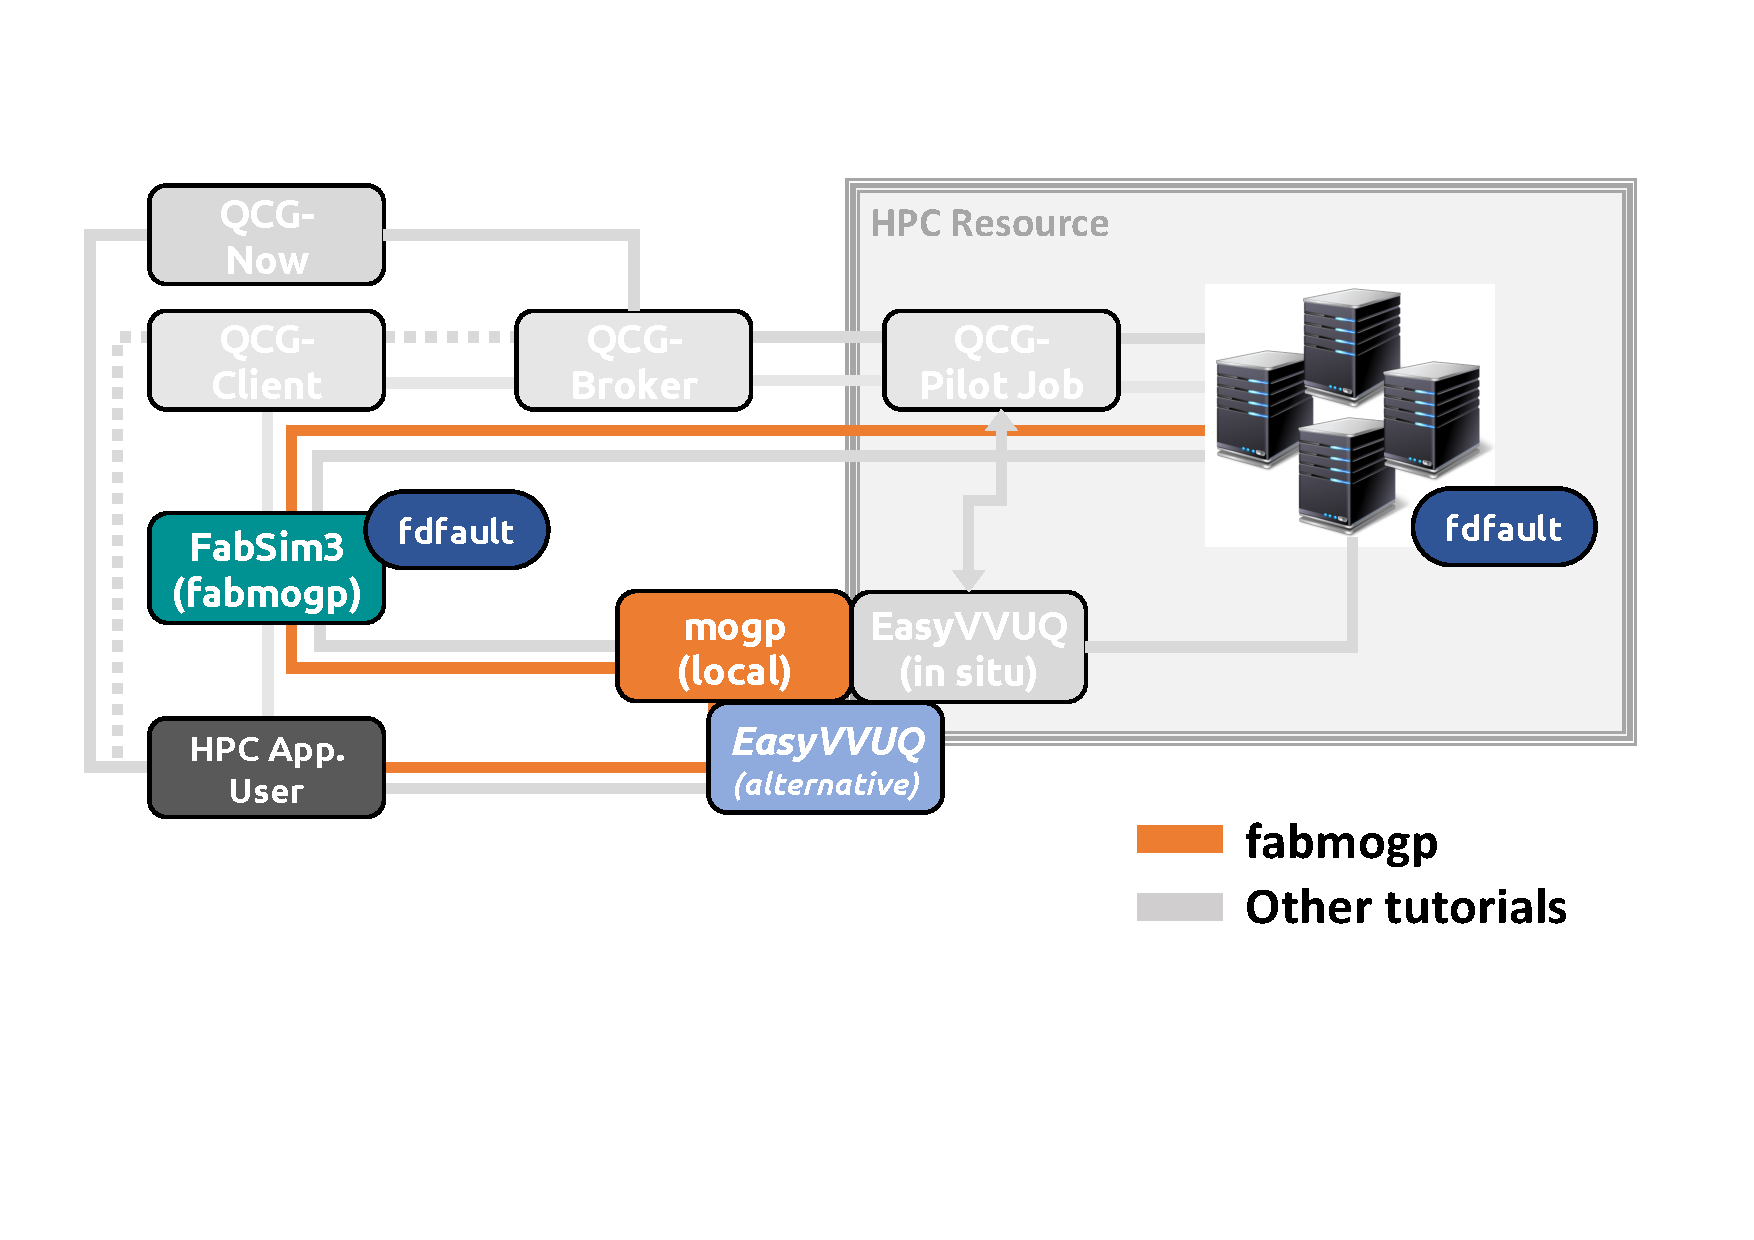
\includegraphics[width=5in]{FabMogpMap.pdf}
\caption{Illustration of the workflow used in our simulations. Local resources are shown on the
left, and remote HPC resources on the right in the light gray box. The HPC user (dark gray box in
the lower left corner) uses a local machine running \texttt{mogp\_emulator} to set up the
UQ workflow. This connects with FabSim3 on the local machine, which is running the
\texttt{fabmogp} plugin. The plugin
connects via SSH to the cluster, where it runs the \texttt{fdfault} simulations (though
in practice, these are actually run locally in our tutorial). FabSim3 collects the results
back on the local machine, where \texttt{mogp\_emulator} performs the surrogate modelling
and history matching.
Other workflows enabled by the VECMA toolkit are shown in light gray on the local machine.}
\label{tubemap}
\end{figure}

FabSim3 is an toolkit for user-developers to help automate computational workflows involving many simulations and remote resources. It has been used in a variety of disciplines, for instance to facilitate coupled atomistic / coarse-grained materials simulations and to perform large-scale sensitivity analysis of agent-based migration models \cite{fabsim}. The tool is open-source (BSD 3-clause license) and one of the main components of the VECMA toolkit.

We conduct our simulations using two FabSim3 simulation tasks: \texttt{mogp\_ensemble}, and
\texttt{mogp\_analysis}.
The \texttt{mogp\_ensemble} workflow will automatically sample the Latin Hypercube to create the desired number of points, set up all of the necessary earthquake simulations, and run them. The advantage of using this approach over the manual approach described above is that the runs are each performed in individual directories, with input, output and environment curated accordingly. This makes it very easy to reproduce individual runs, and also helps with the diagnostics in case some of the simulations exhibit unexpected behaviours.

Additionally, our choice of earthquake simulation has made a number of compromises in order to
ensure that the simulations run in a reasonable amount of time given the constraints of the
workshop format where it was initially presented. However, to make the simulations more realistic
will require additional computational resources. A typical 3D dynamic rupture simulation of a similarly
sized earthquake will usually require tens of hours on 64+ cores, depending
on the exact model setup and simulation approach used. By implementing this workflow using FabSim3,
we are able to test and debug the simulations locally, yet we can easily scale the simulations
up to larger problems in 3D on a cluster without needing to change any of our execution scripts.
This illustrates the utility of using a simulation management tool like FabSim3.

Once the ensemble has run, FabSim3 can automatically fetch the simulation results for analysis. The
analysis to fit the GP emulator and perform History Matching is implemented in a FabSim3 task to
collect the simulation results and perform the UQ workflow. More details are available in the
tutorial text, which is part of the
\texttt{fabmogp} code base.

\section{Results}

\subsection{Simulator Runs}

A sample output from the Latin Hypercube Design with 20 sample points is shown in Table~\ref{table_lhc}.
The input parameters take on a range of values spread out through the entire space, which are converted
into the raw stress values for execution in the \texttt{fdfault} simulation.

\begin{table}[!h]
\caption{Latin Hypercube experimental design samples used for building the surrogate model and the
corresponding integrated slip}
\label{table_lhc}
\begin{tabular}{ccccc}%%%The number of columns has to be defined here
\hline
Normal Stress & Shear/Normal Stress & Normal Stress Ratio & Simulator Output \\
\hline
-120 MPa & 0.25 & 1. & 125. \\
\\\hline
\end{tabular}
\vspace*{-4pt}
\end{table}%%%End of the table

The simulator output is calculated by integrating the final slip at the end of the simulation over the
entire fault plane using Simpson's rule. Because all simulations have the same shear modulus and our
simulations are 2D, we simply use this integrated slip as the simulator output as it is proportional
to the seismic moment. Values range from 35 m km to around 300 m km.

\subsection{Surrogate Model}

From these simulator runs, we fit a Gaussian Process emulator to the outputs using the default
\texttt{mogp\_emulator} parameters. We use the Scipy implementation of L-BFGS-B \cite{lbfgs} to minimise the
negative marginal log-likelihood, and use gradient information as the log-likelihood gradient
can be computed in closed form and requires little computational overhead beyond performing the
Cholesky decomposition that is cached from the log-likelihood computation \cite{gprw}.

Because the hyperparameters are constrained to be positive, we fit the logarithm of the correlation
lengths and overall covariance to convert the problem into an unconstrained optimisation, which tends
to be more stable. The resulting correlation lengths on a linear scale are 1, 1, and 1\unskip,
for the normal stress, shear to normal, and normal stress ratios, respectively.
The overall covariance is 200\unskip, which has also been converted to a linear scale.
The covariance scale matches the range of simulations
output noted in Table~\ref{table_lhc}, and the correlation lengths are of a similar scale to the actual
input values, suggesting that our emulator does a reasonable job of capturing the information in
the simulation outputs.

\subsection{History Matching}

With the fit GP emulator, we can now make predictions using a dense sampling of points drawn from the
experimental design and compare with an observed value using History Matching. We use 10,000 samples
in the analysis that follows. For the sake of this demostration, we simply choose an arbitrary value
from within the range of simulation outputs to serve as our ``observed'' value to illustrate how the
procedure works, though in practice the observed seismic moment would be the size of a particular
earthquake on the fault that is being studied. We assume that there is no error in the true value
and the only uncertainty is the emulator prediction uncertainty to simplify the demonstration, though
in practice the additional uncertainty from the observational error and model discrepancy will simply
expand the size of the space that has not been ruled out.

An example of the samples that have been not ruled out yet (NROY) for the observed value of 58 m km
is shown in Fig.~\ref{fig_nroy} projected into the normal and shear/normal ratio plane of parameter
space. We use a plausibility threshold of 3 standard deviations from the mean to rule out points.
We note that the NROY space is fairly clustered around along a specific curve in this space.
At high compressive normal stresses, this seismic moment is produced for shear/normal stress ratios
of around 0.16, while at lower normal stresses the shear/normal stress must be slightly higher
near 0.2 to
produce the known value. At very low shear to normal stresses there is a region that cannot be
ruled out, though the fact that this occurs near the boundary of the space suggests this may be
an artifact of our original sampling. Designs with more sample points do not exhibit this feature.
We note that the projection shown in Fig.~\ref{fig_nroy} was found to capture most of the structure
in the space, and suggests that the additional normal
stress component is less important for predicting the final seismic moment in our simulations.

\begin{figure}[!h]
\centering\includegraphics[width=4in]{figure2.pdf}
\caption{Points that have not been ruled out yet (NROY) projected into the normal and shear/normal plane of the parameter space. Note that the points are fairly tightly clustered along a line, showing that the earthquake size is very sensitive to the stress tensor components.}
\label{fig_nroy}
\end{figure}

The implausibility metric used to determine the NROY space (Eq.~(\ref{implaus})) is shown in
Fig.~\ref{fig_implausibility}. As we can see, most values that are ruled out have implausibility
metrics much greater than 6, indicating that we have a high degree of confidence that they can be
ruled out. This knowledge allows us to focus further simulation effort and anlysis on a much narrower
part of parameter space, so that future computational effort is focussed on the most likely parameter
values to improve our understanding of the problem and make predictions.

\begin{figure}[!h]
\centering\includegraphics[width=4in]{figure3.pdf}
\caption{Implausibility metric (number of standard deviations between the observation and the predictions of the surrogate model, Eq.~(\ref{implaus})) in the parameter space projected into the normal and shear/normal plane. As with the NROY plot, this shows the sensitivity of the output to the stress components.}
\label{fig_implausibility}
\end{figure}

\section{Conclusion}

This paper and the associated tutorial demonstrate the use of a variety of computational tools
to implement and execute a UQ calibration workflow on a computationally intensive earthquake
model. Our implementation can automate the entire workflow with a few simple command line
instructions, and the FabSim3 plugin facilitates scaling our simulations to more intense
problems requiring execution on a computer cluster. Our implementation also makes the UQ
and earthquake simulation methods accessible to new users and facilitates reproducibility
by providing the computational environment required to run them.
Our results also illustrate how the \texttt{mogp\_emulator} package allows implementation on
robust model calibration approaches on problems that have not previously considered such
an approach. The library allows flexible specification of all components of the calibration
workflow and is easily adaptable to other physical systems.

The UQ results demonstrate that given the seismic moment of an event, we can rule out
much of the input stress parameter space, as the earthquake size is highly sensitive to
the stress. This can potentially overcome one of the main challenges of using dynamic
earthquake modeling for seismic hazard analysis. In Probabilistic Seismic Hazard Analysis \cite{psha},
the standard approach for estimating risk due to strong ground motions, analysts must
first determine the distribution of earthquake sizes expected to occur over a given time period.
This is usually done empirically based on very limited observations, and does not attempt
to determine if such earthquake sizes are consistent with physical models.
Our UQ approach could enable use of dynamic simulations in this approach by providing a set
of NROY points that are consistent with the limited observations, and use those points to
simulate a much more comprehensive set of ruptures consistent with the historical data
to supplement the limited existing strong motion records \cite{gmpe}.
These physical simulations can thus capture the natural variability of events in a region,
something that current empirical approaches cannot do in a physical way.
This will enable
physics-based seismic hazard analysis that exploits simulations in a way not previously
possible, and give more robust estimates of future earthquake sizes and ground motions
in a way that better constrains uncertainties in both the physical models and the
predicted hazard.

\vskip6pt

\enlargethispage{20pt}

\dataccess{
All simulation codes used in this work are publically available on Github under free and open
source software licenses:
\begin{itemize}
   \item \texttt{mogp\_emulator} https://github.com/alan-turing-institute/mogp\_emulator
   \item \texttt{FabSim3} https://github.com/djgroen/fabsim3
   \item \texttt{fdfault} https://github.com/egdaub/fdfault
\end{itemize}
The FabSim3 plugin that implements all of the simulations and analysis described in this work
is also available under a free and open source licese on Github:
\begin{itemize}
   \item \texttt{fabmogp} https://github.com/edaub/fabmogp
\end{itemize}
This repository also contains the associated tutorial to describe this workflow,
the underlying \texttt{mogp\_emulator} code, and the FabSim3 commands can be found in this
repository as well at https://github.com/edaub/fabmogp/blob/master/Tutorial.rst.
The computational
environment and associated scripts and build instructions used to produce the simulations,
figures, and the typeset manuscript is available as a
Docker image in a Github repository. The repository contains detailed instructions on building
and running the simulations is
available at https://github.com/alan-turing-institute/fabmogp\_paper.
}

\aucontribute{EGD designed and implemented the UQ workflow and earthquake simulations. HA, IM and DG
implemented the FabSim3 plugin to carry out this workflow. All authors contributed to writing the
associated tutorial and this manuscript.}

\competing{The author(s) declare that they have no competing interests.}

\funding{EGD received support from EPSRC grant EP/N510129/1HA to the Alan Turing Institute. IM and DG have received funding from the European Union Horizon 2020 research and innovation programme under grant agreement No 800925 (VECMA) and 824115 (HiDALGO).}

\ack{We thank Diana Suleimenova for commments on the tutorial text.}

%%%%%%%%%% Insert bibliography here %%%%%%%%%%%%%%

\bibliographystyle{rsta}
\bibliography{fabmogp_paper}

\end{document}
